\subsection{Structure Generation}
\label{sec:structure-generation}

We first evaluate structure generation alone, following the structure generation phase of the seventh CCDC CSP blind test~\citep{hunnisett2024seventhgeneration}. We measure whether each generative model can recover the experimental structure within a fixed candidate budget, without energy evaluation, relaxation, or ranking.

\textbf{Benchmarks.} We evaluate on six benchmarks: the OXtal Rigid and Flexible sets, with 50 targets each~\citep{jin2025oxtal}; CSP5, CSP6, and CSP7, with 6, 5, and 8 targets, respectively~\citep{bardwell2011fifth,reilly2016sixth,hunnisett2024seventhgeneration}; and CLARI's CSD Teaching Subset, with 773 targets~\citep{battle2010applications,lo2026clari}.

\textbf{Metric and protocol.} Following OXtal~\citep{jin2025oxtal} and CLARI~\citep{lo2026clari}, we report the crystal-level approximate solve rate $\mathrm{Sol}_C$ at candidate budgets of 30 and 1{,}000. A target is considered solved if any candidate is collision-free, at least 8 of 15 molecules are matched, and $\mathrm{RMSD}_{15}<2\text{\AA}$ with COMPACK~\citep{chisholm2005compack}. $\mathrm{Sol}_C$ is the fraction of solved targets. We also report the stricter $\mathrm{Sol}_C^{15/15}$, which requires all 15 molecules to match. For the 30-candidate budget, we follow CLARI's bootstrapping protocol~\citep{lo2026clari}: from each fixed pool of 1{,}000 candidates, we draw 5{,}000 resamples of 30 candidates and average the resulting $\mathrm{Sol}_C$. Full metric definitions are provided in \Cref{app:structure-generation-evaluation}.

\textbf{Baselines.} We compare against OXtal and three CLARI variants: CLARI-M, CLARI-L, and CLARI-H~\citep{jin2025oxtal,lo2026clari}. For a consistent comparison, we re-evaluate the official CLARI checkpoints using the OXtal evaluation protocol, since the two evaluators differ in collision detection and reference-structure selection. See \Cref{app:structure-generation-evaluation} for details.

\textbf{Results.} Across all six benchmarks, \model{} achieves the highest solve rate at both 30- and 1{,}000-candidate budgets under the standard
and strict criteria (\Cref{fig:benchmark-teaser,fig:benchmark-exact,fig:benchmark-teaser-strict,fig:benchmark-exact-strict}),
outperforming the strongest baseline in 23 of 24 settings and tying on the saturated CSP5 result. At 30 candidates, the relative gain
reaches 54.5\% on CSP7 under the standard criterion and 188.0\% on CSP6 under the strict criterion.
\Cref{fig:strict-structure-examples} further demonstrates accurate recovery across diverse molecules and packing motifs.
Full tables are provided in \Cref{app:structure-generation-results}, results with $Z$ sampled from an empirical prior in
\Cref{app:empirical-unit-cell-z}, and aligned structure overlays in \Cref{app:strict-structure-overlays}.


\begin{figure}[t]
  \centering
  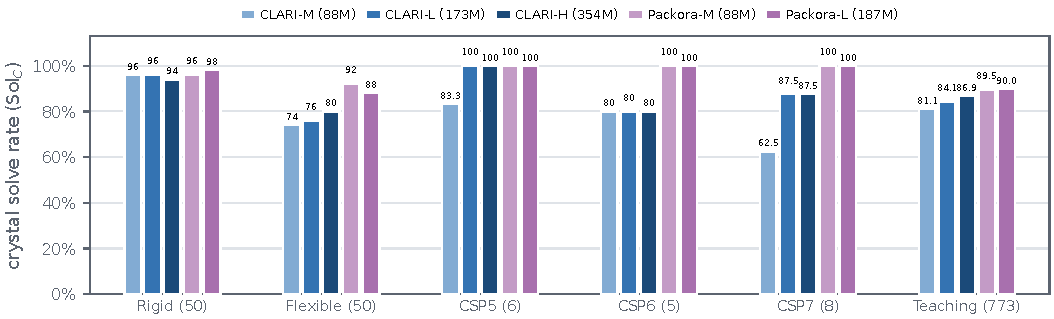
\includegraphics[width=\textwidth]{figures/generated/fig_benchmark_exact.pdf}
    \caption{\textbf{Crystal coverage with 1{,}000 candidates per target.}
    We report the crystal-level solve rate $\mathrm{Sol}_C$ at a generation budget of
    1{,}000 candidates per target. Numbers in parentheses indicate the number of targets in
    each benchmark. \model{} achieves the highest solve rate on all six benchmarks.}
  \label{fig:benchmark-exact}
\end{figure}



\begin{figure}[t]
  \centering
  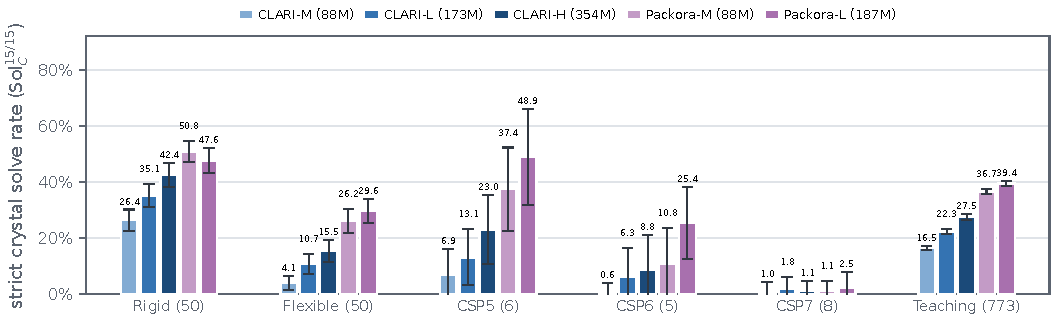
\includegraphics[width=\textwidth]{figures/generated/fig_benchmark_teaser_strict.pdf}
  \caption{\textbf{Crystal coverage with 30 candidates per target under the strict criterion.} We report the crystal-level solve rate $\mathrm{Sol}_C^{15/15}$ at a generation budget of 30 candidates per target. $\mathrm{Sol}_C^{15/15}$ requires all 15
  molecules to match using COMPACK~\citep{bardwell2011fifth}. Numbers in
  parentheses indicate the number of targets in each benchmark. We generate
  1{,}000 candidates per target and report the mean over 5{,}000 bootstrap
  resamples of 30 candidates; error bars show one standard deviation across
  resamples. \model{} achieves the highest solve rate on all six benchmarks.}
  \label{fig:benchmark-teaser-strict}
\end{figure}



\begin{figure}[t]
    \centering
    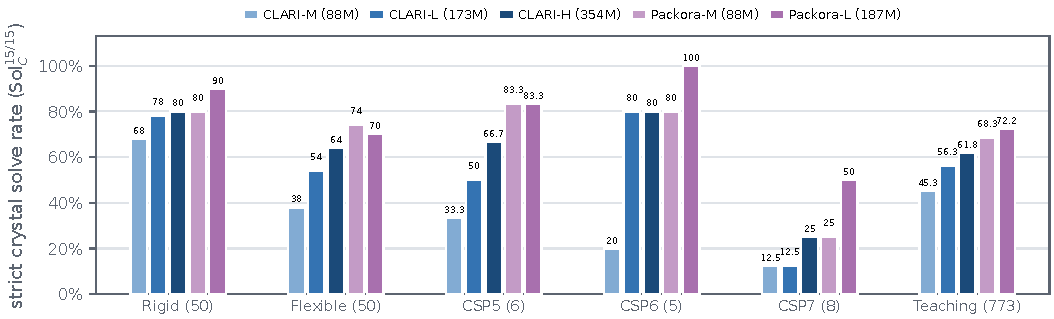
\includegraphics[width=\textwidth]{figures/generated/fig_benchmark_exact_strict.pdf}
    \caption{\textbf{Crystal coverage with 1{,}000 candidates per target under the strict criterion.} We report the crystal-level solve rate $\mathrm{Sol}_C^{15/15}$ at a generation budget of 1{,}000 candidates per target. $\mathrm{Sol}_C^{15/15}$ requires all 15 molecules to match under COMPACK~\citep{bardwell2011fifth}. Numbers in parentheses indicate the number of targets in each benchmark. \model{} achieves the highest solve rate on all six benchmarks.}
    \label{fig:benchmark-exact-strict}
\end{figure}

